\documentclass[12pt, xcolor=beamer,table,usenames,dvipsnames, ignorenonframetext, ngerman]{beamer}
\usetheme{Frankfurt}
\usecolortheme{dove}
\usepackage{appendixnumberbeamer}
%\setbeamersize{text margin left=20pt,text margin right=20pt,}

\beamertemplatenavigationsymbolsempty 
\setbeamertemplate{headline}{}
\setbeamertemplate{itemize item}{\textbullet}

\addtobeamertemplate{navigation symbols}{}{
	\ifnum\insertframenumber>\inserttotalframenumber%
	\relax
	\else%
	\usebeamerfont{footline}%
	\usebeamercolor[fg]{footline}%
	\hspace{1em}%
	\insertframenumber
	\fi%
}
\addtobeamertemplate{frametitle}{\vspace*{.5cm}}{\vspace*{.5cm}}

\setbeamercolor{footline}{fg=black}
\usepackage{soul}
\makeatletter
\let\HL\hl
\renewcommand\hl{%
	\let\set@color\beamerorig@set@color
	\let\reset@color\beamerorig@reset@color
	\HL}

\usepackage{tipa}
\usepackage{tikz}
\usetikzlibrary{shapes.geometric, arrows}
\mode<presentation>

  \setbeamercovered{invisible}
\usepackage{multicol}
\usepackage[english]{babel}
\usepackage[latin1]{inputenc}
\usepackage{times}
\usepackage[T1]{fontenc}
\usepackage{ulem}
\usepackage{tipa}
\usepackage{qtree}
\usepackage{phonrule}
\usepackage{graphicx}
\usepackage{apacite}
\usepackage{xcolor}
\setlength\parindent{0pt}
\usepackage{natbib}
\usepackage{tikz}
\usetikzlibrary{arrows.meta}
\usepackage{tcolorbox}
\tcbuselibrary{raster}

\title{A-maze of Natural Stories: Texts are comprehensible using the Maze task}
\author{Veronica Boyce, Roger Levy}
\date{AMLaP 2020}


\begin{document}

\begin{frame}
\maketitle
%TODO maybe put a picture of Roger's face??, at least acknowledge him 
%Pre-amble -- thank Roger, outline with be methods heavy, and then talk about the specific experiment & how it's relevant to how we think about surprisal 
\end{frame}

% But first -- Incremental processing methods


\begin{frame}{Incremental processing methods}
\pause
Goal: Measure processing difficulty

Assumption: Longer RT = more difficulty
\medskip

\pause
\end{frame}

\begin{frame}{Incremental processing methods}
	How to measure RT?
	
Usual Methods
\begin{columns}[t]\pause
	\begin{column}{.5\textwidth}
		\begin{center}
			\textbf{\Large Eye-tracking}
			
			\medskip
			
			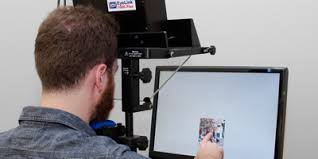
\includegraphics[width=.9\textwidth]{../eye-tracker.jpeg}
			\pause
		\end{center}
	\end{column}\pause
	\begin{column}{.5\textwidth}
		\begin{center}
\textbf{\Large Self-paced reading}

\medskip

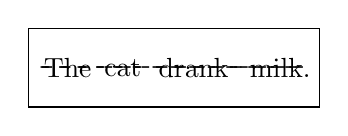
\begin{tikzpicture} %TODO on slide etc
\draw (-.5,-.5) rectangle (3.2,.5);
\onslide<4>{\node at (0,0) {The};}
\onslide<4>{\node at (1.7,0) {- - - - - - - - - - -};}
\onslide<5>{\node at (0,0) {- - - };}
\onslide<5>{\node at (.7,0) {cat};}
\onslide<5>{\node at (2,0) {- - - - - - - - };}
\onslide<6>{\node at (0.3,0) {- - - - - - };}
\onslide<6>{\node at (1.6,0) {drank};}
\onslide<6>{\node at (2.6,0) {- - - -};}
\onslide<7->{\node at (.9,0) {- - - - - - - - - - -};}
\onslide<7->{\node at (2.7,0) {milk.};}
\end{tikzpicture}
\end{center}
\onslide<8->{
}
\end{column}
\end{columns}
\bigskip
Different methods have different trade-offs
\end{frame}

\begin{frame}{An alternative: Maze}
%TODO First mentioned, then more elaborated in 2009 paper, has been used ~dozen times 
\centering
\tikzset{
	font={\fontsize{14pt}{12}\selectfont}}
%TODO Maybe update with circles to show the selections. 
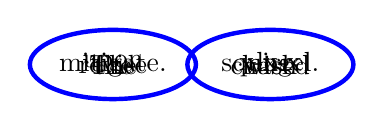
\begin{tikzpicture}
\onslide<1-2>{\node  (c) at (-1,.5) {The};}
\onslide<1-2>{\node  (d) at (1,.5) {x-x-x};}
\onslide<3-4>{\node  (c) at (-1,.5) {upon};}
\onslide<3-4>{\node  (d) at (1,.5) {dog};}
\onslide<5-6>{\node  (c) at (-1,.5) {revise};}
\onslide<5-6>{\node  (d) at (1,.5) {chased};}
\onslide<7-8>{\node  (c) at (-1,.5) {the};}
\onslide<7-8>{\node  (d) at (1,.5) {wish};}
\onslide<9-10>{\node  (c) at (-1,.5) {mitigate.};}
\onslide<9-10>{\node  (d) at (1,.5) {squirrel.};}
\onslide<2,8>{\node[ultra thick, draw=blue, ellipse, minimum width=60pt, minimum height= 25pt,align=center] at (c) {};}
\onslide<4,6,10>{\node[ultra thick, draw=blue, ellipse, minimum width=60pt, minimum height= 25pt,
align=center] at (d) {};}
\end{tikzpicture}
\end{frame}

\begin{frame}{An alternative: Maze}
\begin{columns}
	\begin{column}{0.5\textwidth}
		\begin{center}
		\textbf{\large G-maze}
		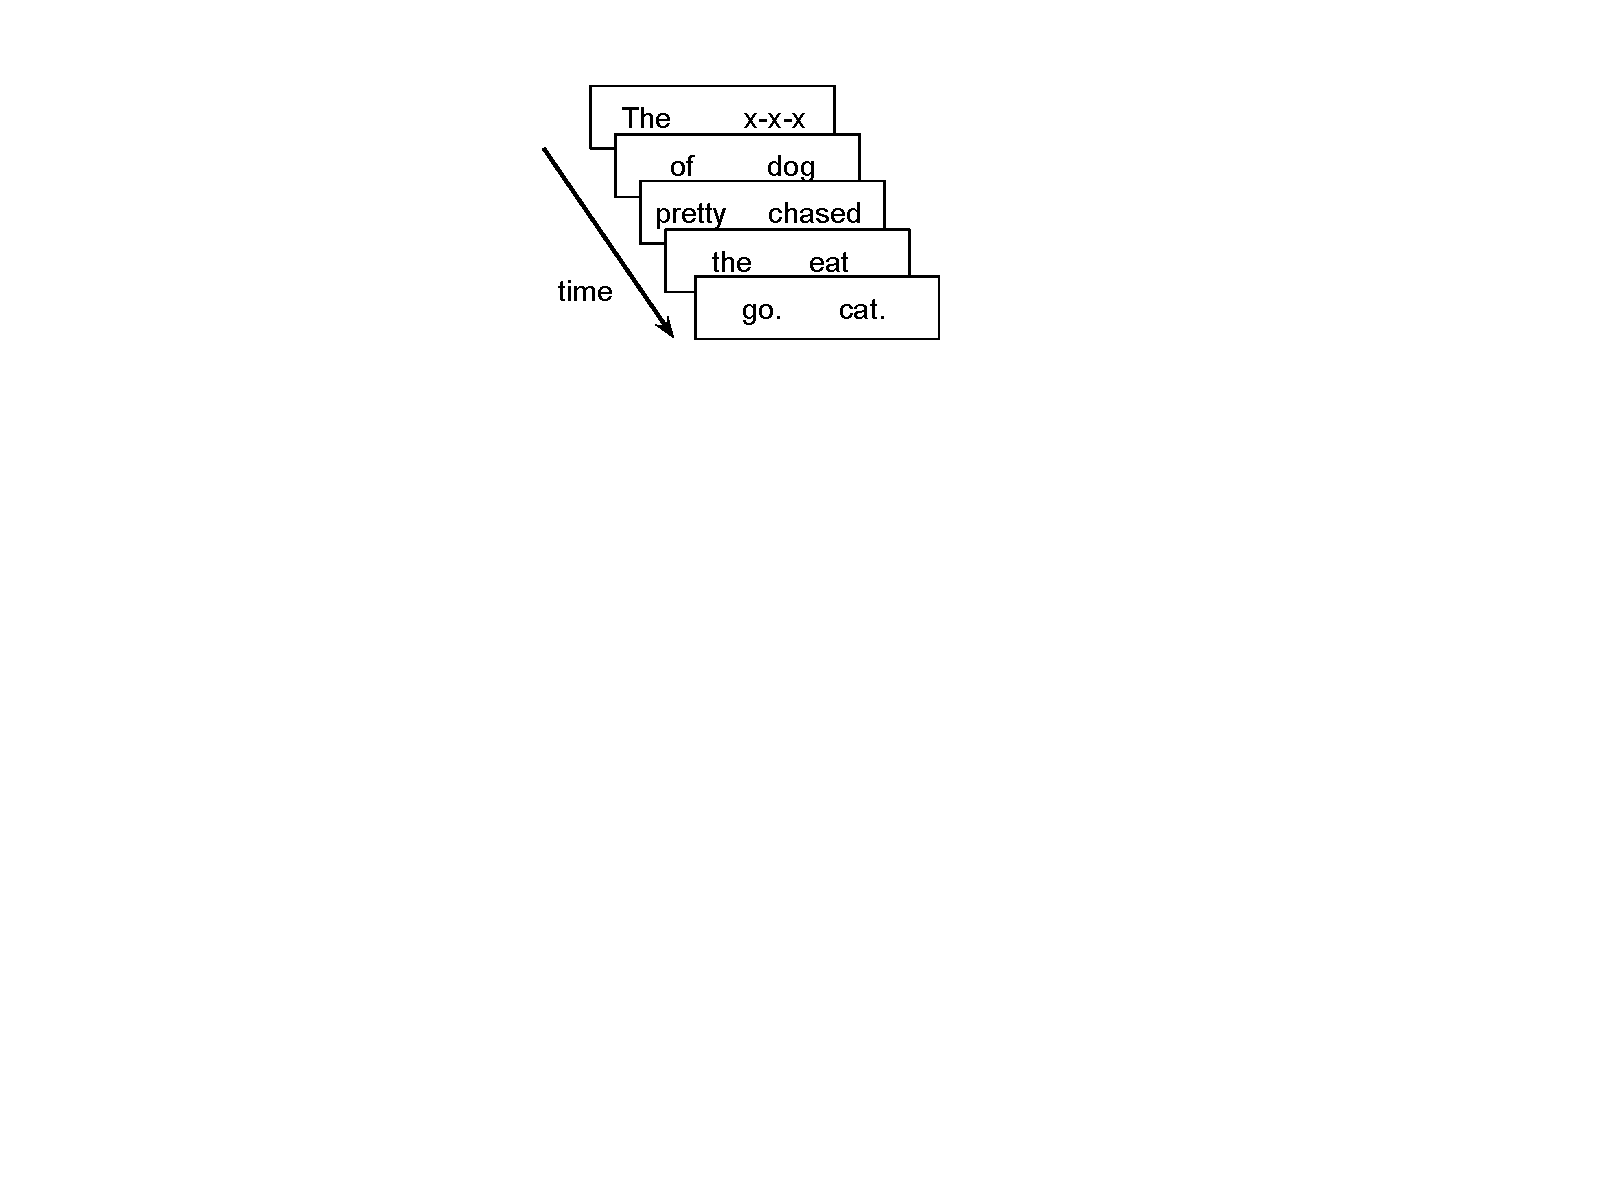
\includegraphics[clip, trim=9cm 14cm 11cm 1cm,width=.9\textwidth]{../gmaze.pdf}
		\end{center}
	\pause
	\end{column}
	\begin{column}{0.5\textwidth} 
		\begin{center}
		\textbf{\large L-maze}
			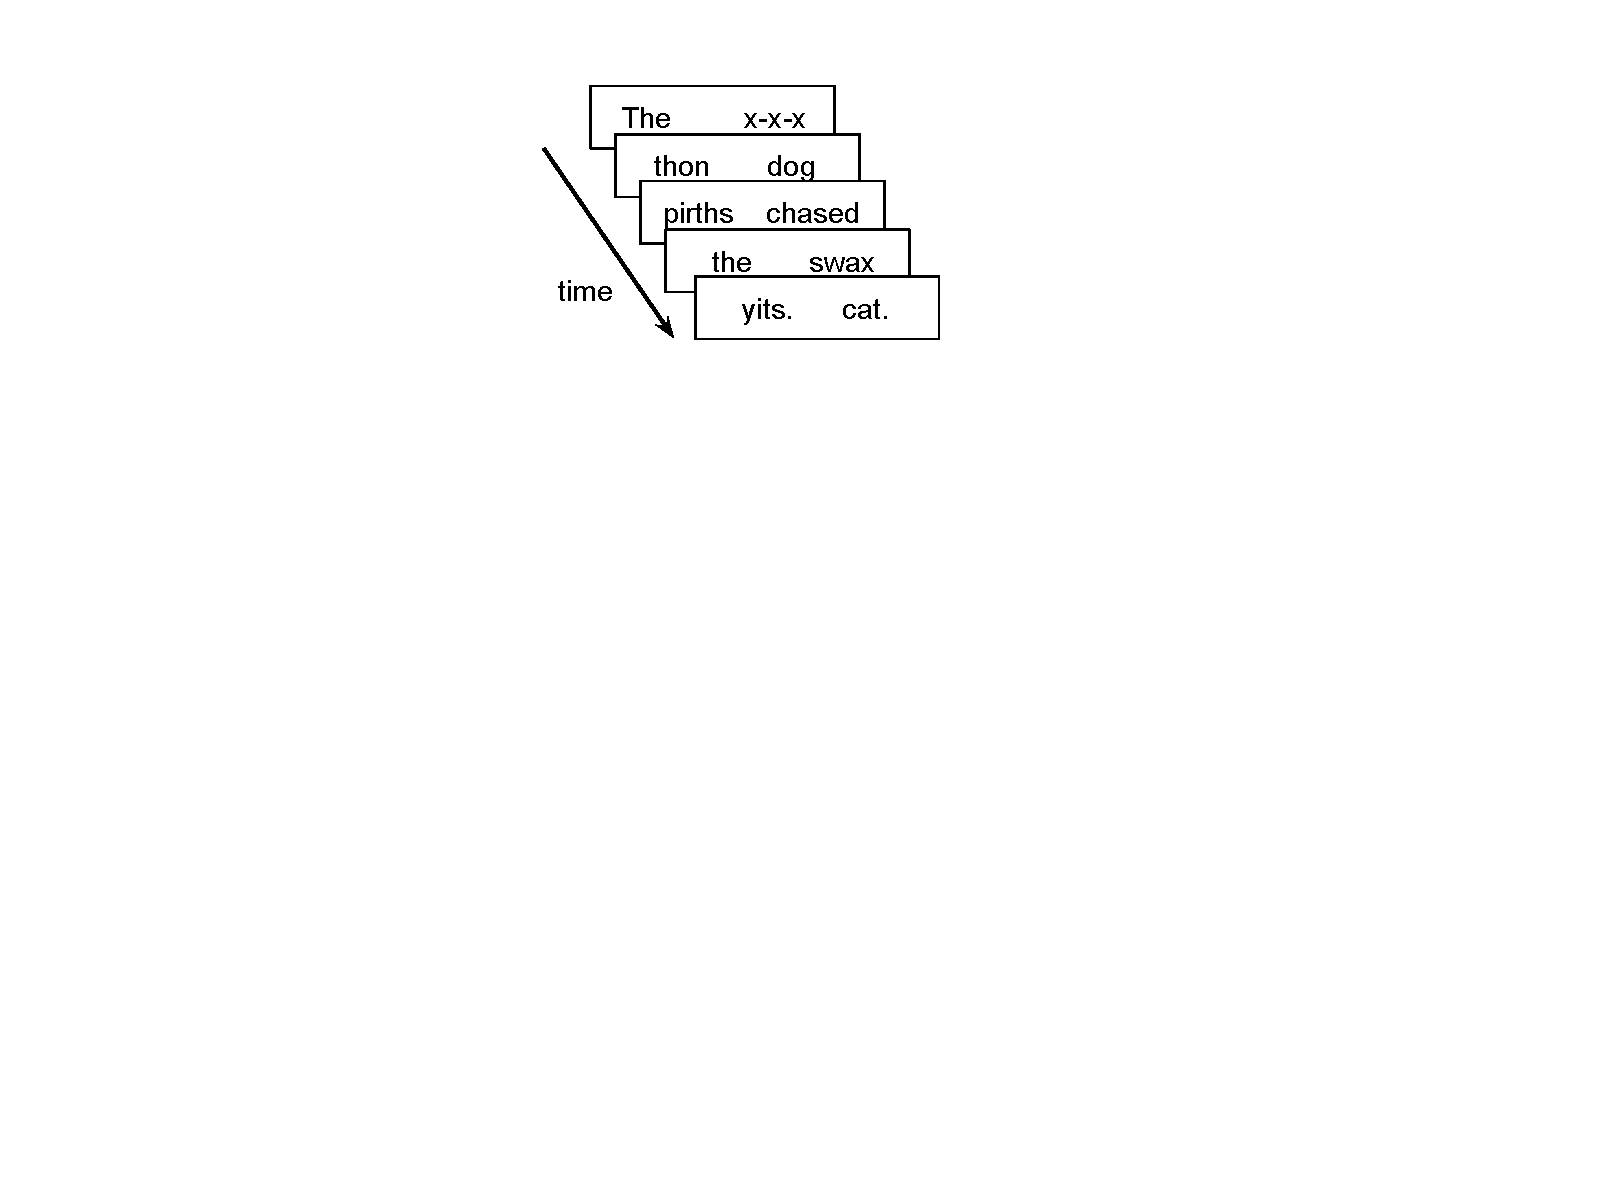
\includegraphics[clip, trim=9cm 14cm 11cm 1cm,width=.9\textwidth]{../lmaze.pdf}
		\end{center}
	\end{column}
\end{columns}

\medskip
\pause
Sentence ends if a mistake is made.
\pause

Claim: forces incremental processing (no spillover)

\begin{flushright}
	{\small(Forster et al. 2009; Witzel et al. 2012)}
\end{flushright}
% Compelling results especially for G-maze, but 
% was run in the lab, and generating G-maze materials is a huge amount of work
\end{frame}

\begin{frame}{Using Maze}
Is Maze a viable alternative to web SPR?

Needs:
\begin{itemize}
	\item Run on web 
	\item Easy generation of distractor words
	\item Work for long or multi-sentence items %this part incidentally makes it easy to do exclusions, and might help with data loss, but we'll talk about that later
\end{itemize} 
\pause

\end{frame}

\begin{frame}{Run on web}
	%TODO include screenshot
	Wrote an Ibex module
	\begin{itemize}
		\item Based off SPR module
		\item Fits in with existing workflow
	\end{itemize}
 Replicated Witzel et al. (2012) results (see Boyce et al. 2020)
\end{frame}
%
\begin{frame}{Using Maze}
	Is Maze a viable alternative to web SPR?
	
	Needs:
	\begin{itemize}
		\item Run on web 
		\item Easy generation of distractor words
		\item Work for long or multi-sentence items %this part incidentally makes it easy to do exclusions, and might help with data loss, but we'll talk about that later
	\end{itemize} 
	\pause
	
\end{frame}
%
\begin{frame}{Generating distractors}
\pause
Task: Given  \textit{The dog chased} Find a word that can't be a continuation.
\begin{itemize}
	\item Tedious (and hard!) to do by hand. 
\end{itemize}

What makes something an unacceptable continuation?
\begin{itemize}
	\item Ungrammatical
	\item ...or otherwise really unlikely 
	\item $\approx$ high surprisal 
\end{itemize}

Can we use Neural Language Models?
\end{frame}
%
\begin{frame}{Can we use LMs?}
Language models (LMs)
\begin{itemize}
	\item Trained on large corpora to predict the next word
	\item Given a partial sentence, return probabilities of the next word
\end{itemize}

LSTM RNNs (ex. Gulordava 2018) show some syntactic knowledge %TODO cite people

Add some controls:
\begin{itemize}
\item Restrict to a list of possible distractors
\item Only consider length, frequency matches
\end{itemize}
	
\end{frame}
%
\begin{frame}{Can we use LMs to choose distractors?} 

Does it work? 

Yes, at least well enough.
\begin{itemize}
	\item Sometimes generates plausible distractors.
	\item Overall results comparable with G-maze %TODO citations to me, Sloggett
	%TODO show graph from Boyce et al
\end{itemize} 
\medskip

Parameter-tweaking may help, as would hand-checking. 
\end{frame}
%
\begin{frame}{Using Maze}
	Is Maze a viable alternative to web SPR?
	
	Needs:
	\begin{itemize}
		\item Run on web %TODO figure out how to make checkmarks again
		\item Easy generation of distractor words 
		\item Work for long or multi-sentence items %this part incidentally makes it easy to do exclusions, and might help with data loss, but we'll talk about that later
	\end{itemize} 
	\pause
	
\end{frame}
%
%
\begin{frame}{Long items}
	
Errors terminate sentences. 
Some error rate is inevitable. 

Want to run multi-sentence items. 
\begin{itemize}
	\item Treat whole story as a unit: Almost no one makes it to the end.
	\item Treat each sentence as a unit:
	Many participants miss key context. 
\end{itemize}

What if after an error, participants corrected errors and the sentence continued?
	
\end{frame}
%
\begin{frame}{Maze with Error Correction}
\centering
\tikzset{
	font={\fontsize{14pt}{12}\selectfont}}

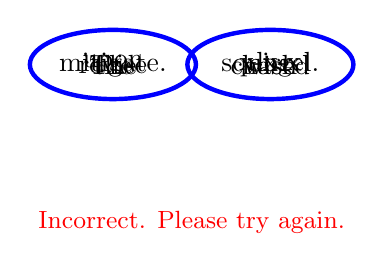
\begin{tikzpicture}
\onslide<1-2>{\node  (c) at (-1,.5) {The};}
\onslide<1-2>{\node  (d) at (1,.5) {x-x-x};}
\onslide<3-4>{\node  (c) at (-1,.5) {upon};}
\onslide<3-4>{\node  (d) at (1,.5) {dog};}
\onslide<5-8>{\node  (c) at (-1,.5) {revise};}
\onslide<5-8>{\node  (d) at (1,.5) {chased};}
\onslide<9-10>{\node  (c) at (-1,.5) {the};}
\onslide<9-10>{\node  (d) at (1,.5) {wish};}
\onslide<11-12>{\node  (c) at (-1,.5) {mitigate.};}
\onslide<11-12>{\node  (d) at (1,.5) {squirrel.};}
\onslide<2,6,10>{\node[ultra thick, draw=blue, ellipse, minimum width=60pt, minimum height= 25pt,align=center] at (c) {};}
\onslide<4,8,12>{\node[ultra thick, draw=blue, ellipse, minimum width=60pt, minimum height= 25pt,
	align=center] at (d) {};}
\onslide<7,8>{\node[text=red] at (0,-1.5) {\small Incorrect. Please try again.};}
\end{tikzpicture}

\end{frame}

\begin{frame}{Maze with Error Correction}

\begin{columns}
	\begin{column}{0.3\textwidth}
		\begin{center}
		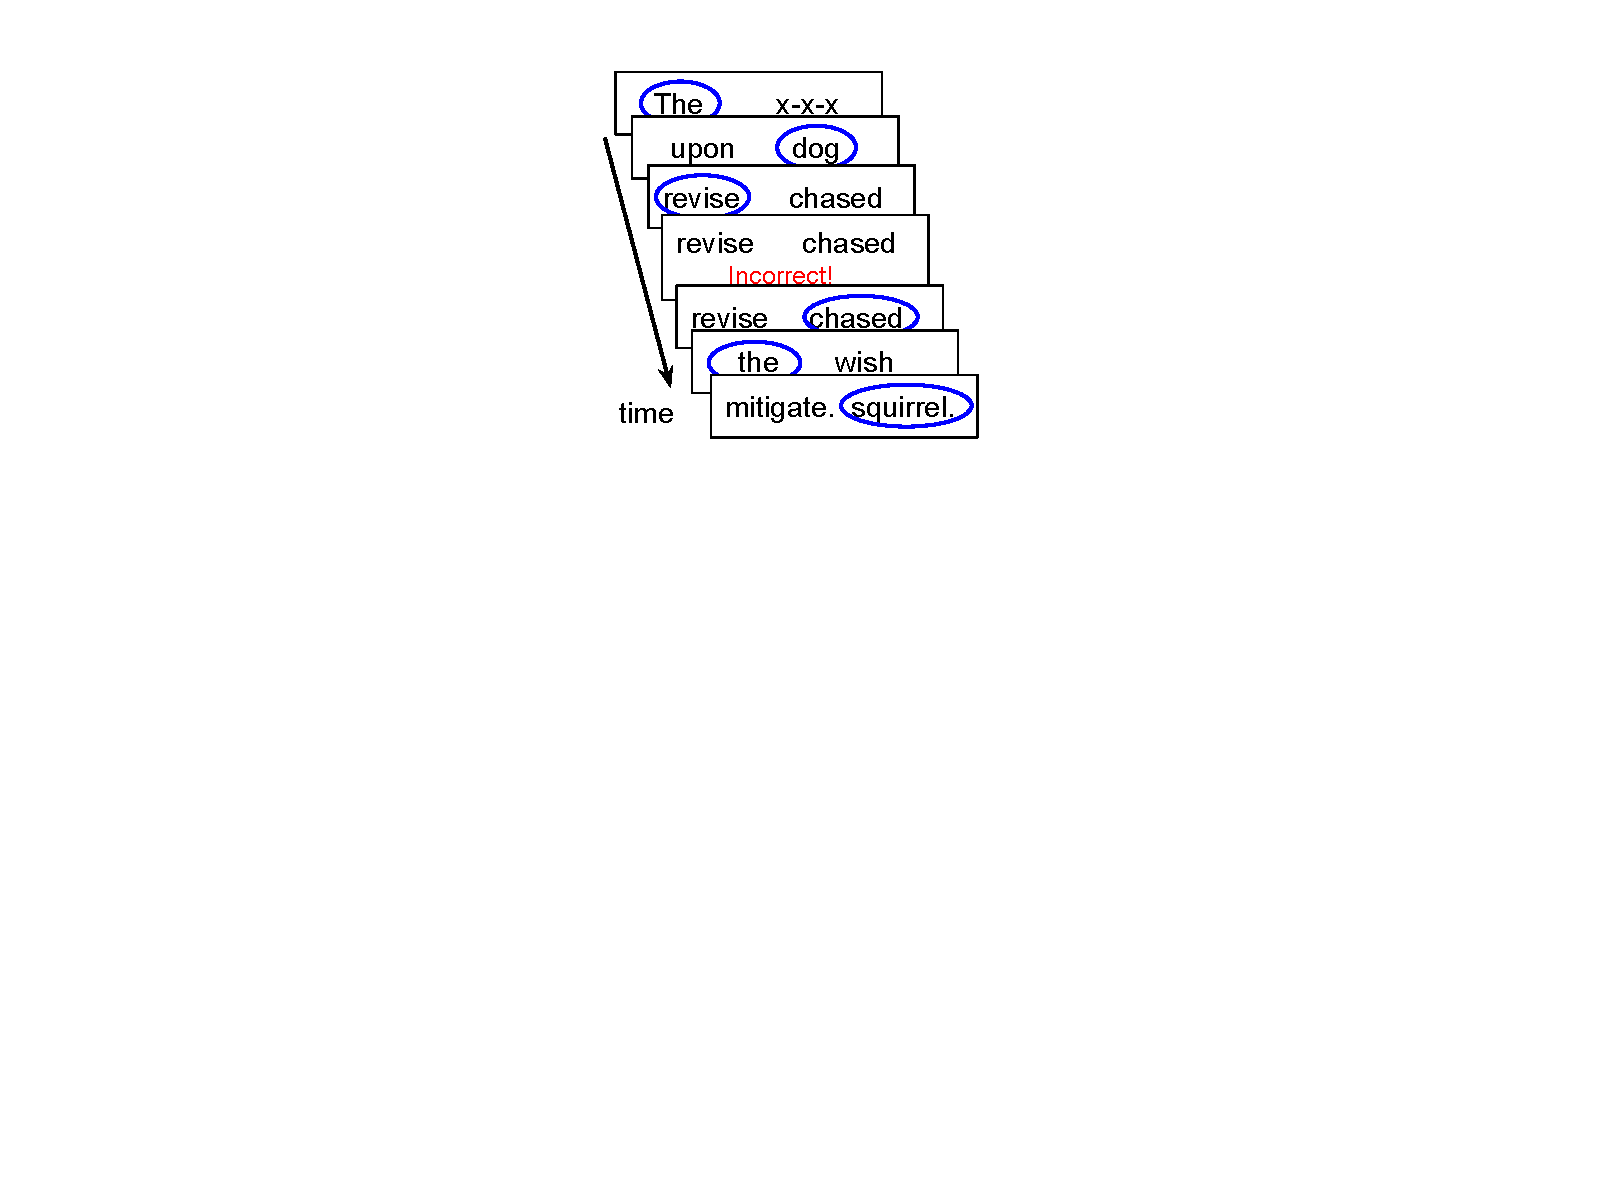
\includegraphics[clip, trim=9cm 12.5cm 10cm 1cm,width=\textwidth]{../maze_diagram.pdf}
		\end{center}
		
	\end{column} \pause 
	\begin{column}{0.7\textwidth} 
		\begin{center}
			Features
			\begin{itemize}
				\item Easily implemented as a toggle in Ibex \pause
				\item Can look at long materials (in principle)
				\item Have all the data \pause
				\item Identify bad participants v bad distractors 
				%easy to weed out participants who aren't paying attention 
				\item Makes it less of a big deal when we have bad distractors
			\end{itemize}
		\end{center}
	\end{column}
\end{columns}
\medskip
\pause

Side effect: Can now run multi-sentence items!
\end{frame}
%
%%So now that I've explained the method, going to switch over to current experiment & what we hoped to get from it
%
\begin{frame}
	Various open questions we want to address -- really test suitability of Maze
	\begin{itemize}
		\item Do people comprehend/remember what they read?
		\item Does this error correction thing work? 
		\item Are people willing to read texts in this way? 
		\item Do we get predictability effects? (Both SPR, eye-tracking show certain surprisal effects, does Maze?)
	\end{itemize}
\end{frame}

\begin{frame}{Natural Stories}
Natural stories corpus (Futrell et al. 2017)
\begin{itemize}
	\item 10 stories, each about 1000 words
	\item Some unusual constructions, but read fluently
	\item 6 comprehension questions per story
\end{itemize}

\end{frame}

\begin{frame}{Natural Stories}

\begin{small}Tulip mania was a period in the Dutch Golden Age during which contract prices for bulbs of the recently introduced tulip reached extraordinarily high levels and then suddenly collapsed. At the peak of tulip mania in February sixteen thirty-seven, tulip contracts sold for more than ten times the annual income of a skilled craftsman. It is generally considered the first recorded economic bubble. [...]
\medskip

Q: When did tulip mania reach its peak?

A: \hspace{3em} 1630's\hspace{3em} 1730's \end{small}

%HARD mode 

\end{frame}

\begin{frame}{Participant accuracy}
100 participants from MTurk each read 1 story (20 minutes) \pause
\begin{center}
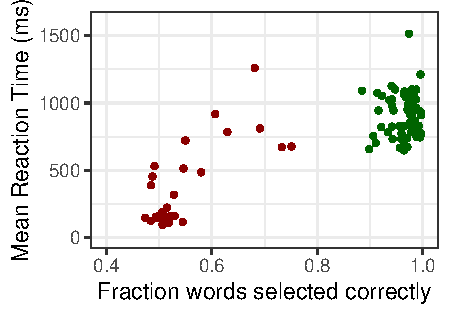
\includegraphics[width=.8\textwidth]{../error.pdf}
\end{center}
\end{frame}
\begin{frame}{Comprehension questions}
\begin{center} \pause
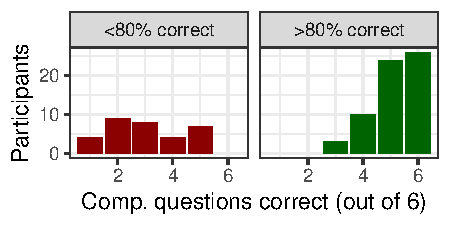
\includegraphics[width=.8\textwidth]{../comp.pdf}
\end{center}
% exclusion options: use comprehension checks as participant filter. Here we can use overall accuracy as the "paying attention" filter. Don't have to worry about how to write good comprehension questions. May still need to do RT exclusions for double-presses or getting distracted. 
\end{frame}



\begin{frame}{Surprisal Effects}
%TODO copy from updated abstract
Use 3 LMs to estimate surprisal: smoothed 5-gram, Gulordava RNN, Transformer-XL (Gulordava et al. 2018, Dai et al. 2019)
\pause

%TODO make sure that updated correct gams are used!!!

Fit GAMs on pre-error data.
\begin{itemize}
	\item Limit to single-token words.
	\item Fit to both current and past word surprisal.
\end{itemize}

\end{frame}

\begin{frame}
	Implications for surprisal theory -- size of the effects is different
	include effect sizes
	Is it about participant quality?
\end{frame}

\begin{frame}{Surprisal Effects}
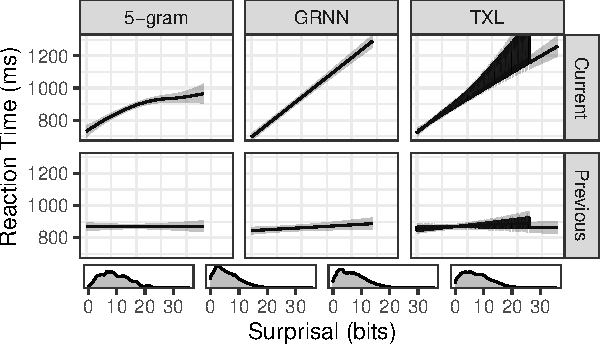
\includegraphics[width=.9\textwidth]{../gam.pdf}	
\end{frame}
\begin{frame}{What about post-mistake data?}
Exclude data from mistakes or the two words after a mistake. 

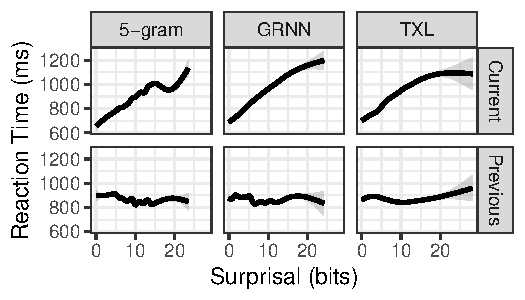
\includegraphics[width=.9\textwidth]{../gam2.pdf}	
\end{frame}

\begin{frame}{Summary}
\begin{itemize}\pause
	\item People will read in the Maze task for 15-20 minutes \pause
	\item It's possible to comprehend during Maze \pause
	\item Distractors are generally good enough \pause
	\item Find expected RT patterns \pause
	\item Very little spillover
\end{itemize}
\end{frame}


\begin{frame}{Use A-maze!}
Easy to use! \pause
\begin{itemize}
	\item Runs on command line \pause
	\item Match distractors across minimal pair sentences \pause
	\item Customize surprisal thresholds, vocabulary lists \pause
	\item Can output pre-formatted for Ibex
\end{itemize}
\medskip
\end{frame}

\begin{frame}{Use A-maze!} \pause
Contribute to A-maze:
\begin{itemize}
	\item Written in Python 3 \pause
	\item Interface with other language models \pause
	\item Add more frequency sources \pause
	\item Extend to non-English languages
\end{itemize}

\end{frame}


\begin{frame}{}

\textcolor{ForestGreen}{\large Documentation: vboyce.github.io/Maze}

with links to the following:
\begin{itemize}

\item A-maze code: github.com/vboyce/Maze

\item Web-maze code: github.com/vboyce/Ibex-with-Maze

\item Sample task: syntaxgym.org:666

\item Paper: psyarxiv.com/b7nqd/
\end{itemize}
\end{frame}


\appendix

\begin{frame}{Matching distractors}
If unspecified: Match by position
\begin{itemize}
	\item The son of the lady who politely introduced \sethlcolor{green} \hl{herself}\sethlcolor{pink} / \hl{himself} was popular at the party.
\end{itemize}
Can specify labels for each word to pair (within item)
\begin{itemize}
	\item The cat who the dog scared hid in a box.\\pre-1 pre-2 who art noun verb main-verb post-1 post-2 post-3
\item The dog who scared the cat sniffed around the couch.\\ pre-1 pre-2 who verb art noun main-verb post-1 post-2 post-3
\end{itemize}
\end{frame}
%%back pocket on more on model results??
%%do we even need back pockets??

\begin{frame}{Post-mistake only}
Exclude data from mistakes or the two words after a mistake. 


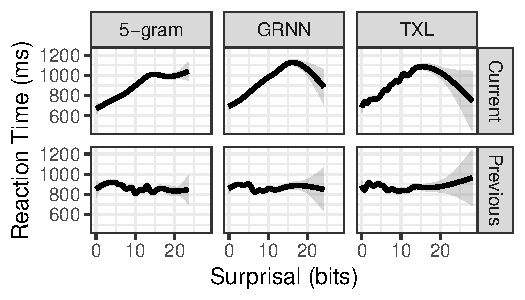
\includegraphics[]{../gam3.pdf}	
\end{frame}

\begin{frame}{Regression coefficients}
\begin{tiny}
\begin{tabular}{l|rlr|rlr|rlr}
	\hline
	&\multicolumn{3}{c|}{5-gram}&\multicolumn{3}{c|}{GRNN}&\multicolumn{3}{c}{TXL}\\
	& Est & CI & $p$ & Est & CI & $p$ &Est & CI & $p$ \\ 
	\hline
	Intercept & 865.3 & [829.9, 902.9] & 0.00 & 871.1 & [837.9, 905.3] & 0.00 & 870.8 & [832.5, 907.8] & 0.00 \\ 
	Surprisal & 11.7 & [9.3, 14.1] & 0.00 & 23.7 & [21, 26.5] & 0.00 & 18.5 & [16.1, 21.1] & 0.00 \\ 
	Frequency & -2.9 & [-6.3, 0.5] & 0.10 & 2.9 & [-0.2, 6] & 0.06 & 0.4 & [-2.7, 3.5] & 0.79 \\ 
	Length & 20.5 & [15.4, 25.6] & 0.00 & 18.5 & [13.3, 23.7] & 0.00 & 21.4 & [16.2, 26.6] & 0.00 \\ 
	Surprisal:Length & -2.0 & [-3, -1] & 0.00 & -1.8 & [-2.7, -0.9] & 0.00 & -1.4 & [-2.2, -0.6] & 0.00 \\
	Freq:Length & -1.0 & [-2.5, 0.4] & 0.16 & -0.1 & [-1.2, 1] & 0.82 & 0.2 & [-0.9, 1.2] & 0.76 \\ 
	\hline
	Past Surprisal & 1.6 & [-0.5, 3.6] & 0.14 & 2.7 & [0.8, 4.5] & 0.00 & 0.8 & [-0.9, 2.5] & 0.40 \\ 
	Past Freq & 2.6 & [-0.1, 5.4] & 0.06 & 1.9 & [-0.2, 4.2] & 0.08 & 1.2 & [-1.1, 3.6] & 0.30 \\ 
	Past Length & -4.8 & [-9, -0.1] & 0.04 & -6.6 & [-10.9, -2.1] & 0.00 & -5.2 & [-9.3, -0.7] & 0.03 \\ 
	Past Surp:Length & -0.2 & [-1.2, 0.8] & 0.72 & -0.9 & [-1.7, -0.2] & 0.01 & -0.6 & [-1.3, 0.2] & 0.13 \\ 
	Past Freq:Length & -1.0 & [-2.3, 0.3] & 0.15 & -1.8 & [-2.9, -0.8] & 0.00 & -1.5 & [-2.6, -0.5] & 0.01 \\ 
	
	
	
	
	\hline
\end{tabular}
\end{tiny}
\end{frame}


\end{document}

